\begin{figure}[H]

	\centering
	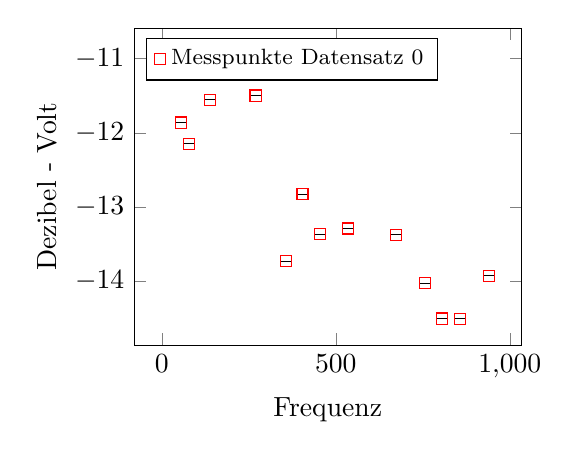
\begin{tikzpicture}
		\pgfplotsset{width=6.5cm,compat=1.3,legend style={font=\footnotesize}}
		\begin{axis}[xlabel={Frequenz},ylabel={Dezibel - Volt},legend cell align=left,legend pos=north west]
		
\addplot+[only marks,color=red,mark=square,error bars/.cd,x dir=both,x explicit,y dir=both,y explicit,error bar style={color=black}] table[x=X,y=Y,x error=xerror,y error=yerror,row sep=\\]{
			X	Y	xerror	yerror	\\
			 13.183594 	 -10.945357 	 0 	 0 	\\
			 55.664062 	 -11.861673 	 0 	 0 	\\
			 77.636719 	 -12.146492 	 0 	 0 	\\
			 139.160156 	 -11.552087 	 0 	 0 	\\
			 269.53125 	 -11.497283 	 0 	 0 	\\
			 357.421875 	 -13.733462 	 0 	 0 	\\
			 404.296875 	 -12.828142 	 0 	 0 	\\
			 455.566406 	 -13.365859 	 0 	 0 	\\
			 536.132812 	 -13.290147 	 0 	 0 	\\
			 672.363281 	 -13.373598 	 0 	 0 	\\
			 757.324219 	 -14.028664 	 0 	 0 	\\
			 805.664062 	 -14.504683 	 0 	 0 	\\
			 856.933594 	 -14.506615 	 0 	 0 	\\
			 940.429687 	 -13.92639 	 0 	 0 	\\
		};
		\addlegendentry{Messpunkte Datensatz 0}

		\end{axis}
		\end{tikzpicture}
	\caption{Umgebung}
	\label{fig:Umgebungsmessung}
\end{figure}
